\chapter{Vorgehensweise}
\label{sec:vorgehensweise}

Wie jedes Projekt benötigt auch die Erstellung des Prototypen der neuen Hochschul-\ac{App} eine Vorgehensweise, nach der das Entwicklerteam geordnet arbeiten kann. Hierbei stellt sich vor allem die Frage, welches Vorgehen bei einer Teamgröße von zwei festen Entwicklern und einem Auftraggeber sinnvoll anzuwenden ist. Deshalb wurde im Rahmen dieses Projektes eine Abwandlung des bekannten \textit{Scrum}-Vorgehensmodells angewendet. Die genaue Umsetzung dieser Abwandlung soll im folgenden nur kurz angedeutet werden, um einen Einblick zu verschaffen, wie die Ergebnisse aus dem Rest der Arbeit erstellt wurden.

\section{Grundkonzept}

Die Idee hinter \textit{Scrum} liegt darin, eine flexible Zusammenarbeit zwischen Kunden und Entwicklern zu ermöglichen. Dabei muss am Anfang eines jeden Projektes eine Sammlung aus Anforderungen in technische Aufgaben umgewandelt werden. Diese Sammlung heißt dann \textit{Backlog}. Danach werden Entwicklungsphasen in sogenannte \textit{Sprints} aufgeteilt, die nicht länger als zwei bis drei Wochen andauern sollten. In diesen Sprints werden Aufgaben aus diesem \textit{Backlog} übernommen. In der Regel sind die Aufgaben untereinander priorisiert, weshalb die ersten Sprints auch die wichtigsten Funktionen implementieren sollten. Während der Sprints können die Aufgaben im \textit{Refinement} nochmals angepasst werden und Fragen an den Auftraggeber können hier nochmals adressiert werden. Am Ende eines jeden Sprints werden die Ergebnisse im sogenannten \textit{Sprint Review} nochmals evaluiert und dann als abgeschlossen markiert, worauf im nächsten Sprint neue Aufgaben aufgenommen werden können.

\section{Umsetzung}

Die Anpassung dieses Konzepts liegt grundlegend darin, dass die Rolle des Auftraggebers hier nicht vom eigentlichen Auftraggeber gespielt wurde, sondern vom Entwicklerteam als Ganzes. Immer wenn Entscheidungen getroffen werden mussten, mussten beide Entwickler zu einer gemeinsamen Antwort kommen. Die Sprint Refinements konnten deutlich vereinfacht werden, da lediglich die Kommunikation zwischen zwei Entwicklern nötig war und die Sprint Reviews so am Ende jeden Sprints als kurzes Treffen abgehalten werden konnte. Im folgenden sollen die wichtigsten Phasen und Aufgaben aus dem Vorgehen kurz erläutert werden. Für die Planung und Dokumentation der Sprints wurde die Online-Plattform \textit{Trello} genutzt, die das Erstellen von agilen Sprint-Boards sehr einfach gestaltet\autocite[][]{trello}. Das \textit{Scrum Board}, das dabei erstellt wurde, sieht wie folgt aus:

\begin{figure}[H]
\centering
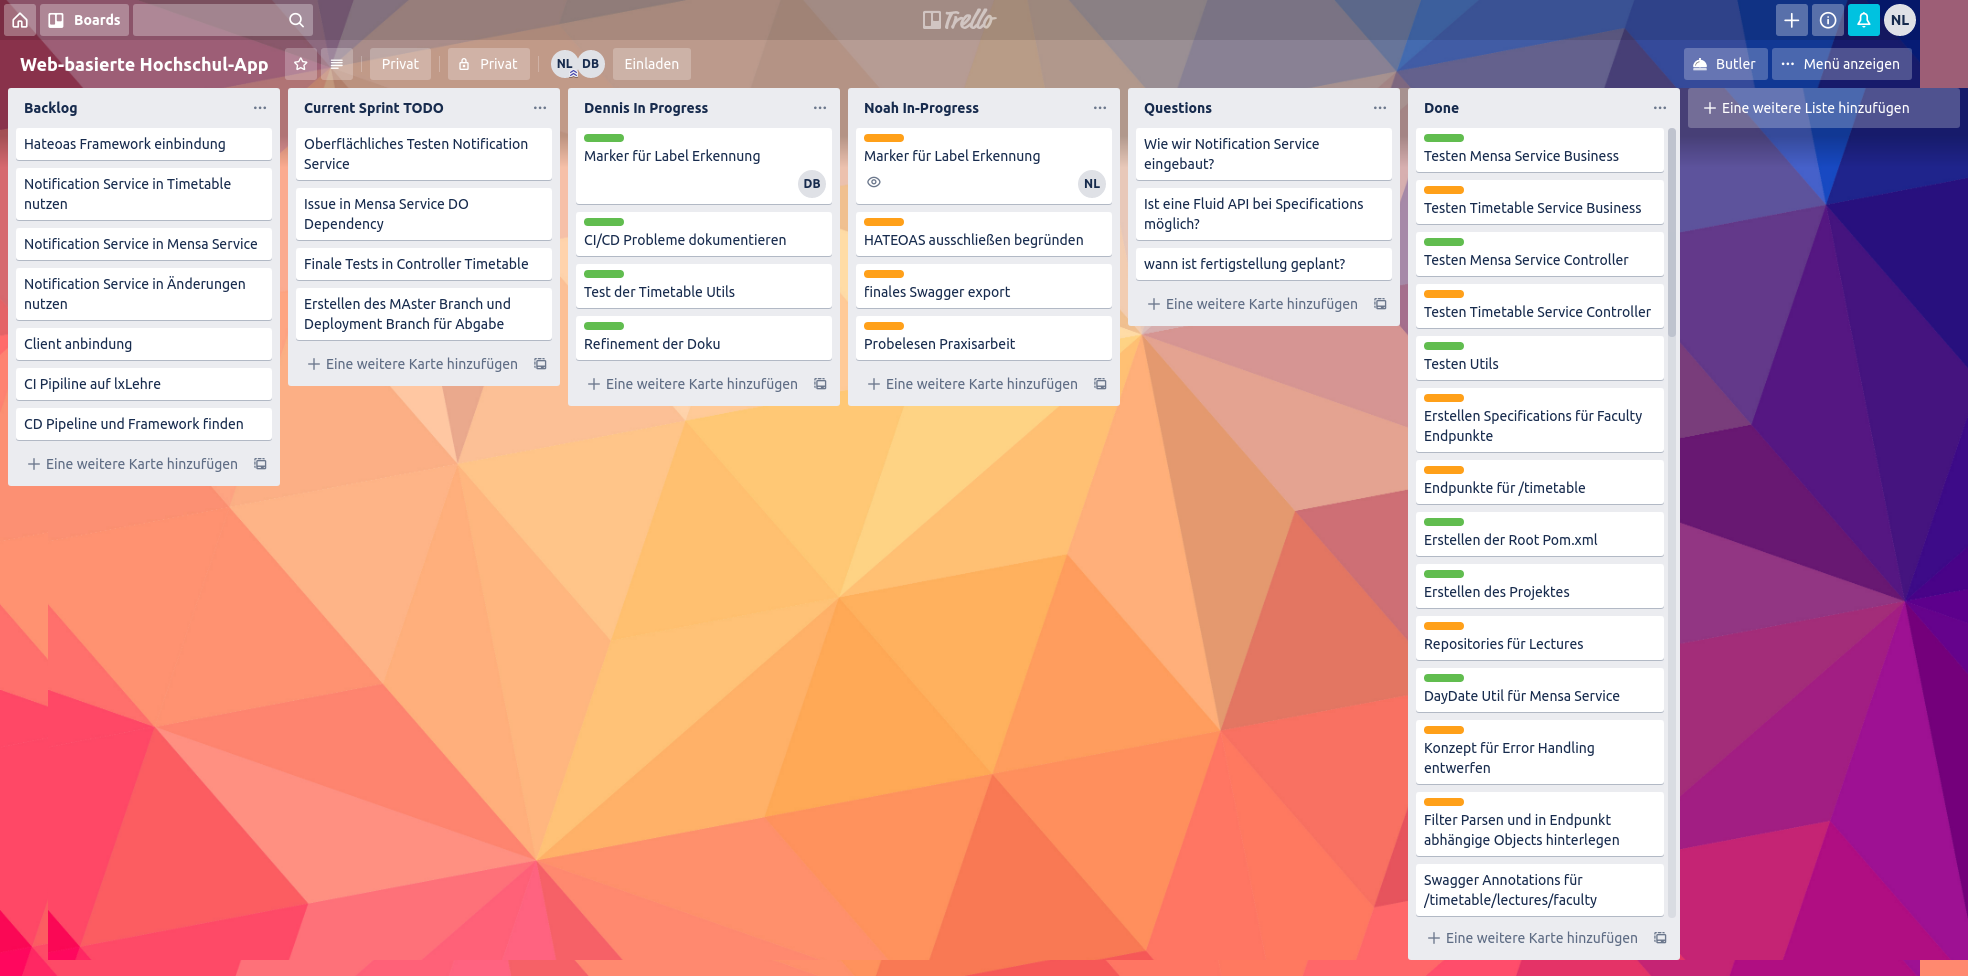
\includegraphics[width=\pictureWidth cm + 2 cm]{Bilder/Kapitel_2/trello_board.png}
\caption{Agiles Trello Board\label{fig:trello_board}}
\end{figure}

\subsection*{Sammeln der Anforderungen}

In der parallel zu dieser Arbeit erstellten Bachelorarbeit wurde bereits ein umfassendes Lastenheft erstellt, welches die funktionalen Anforderungen sammelt und kategorisiert. Anhand dieses Lastenhefts wurde ein Pflichtenheft \footnote{Siehe Anhang \ref{tab:lastenheft}} erstellt, aus dem dann die technischen Aufgaben abgeleitet wurden, welche dann in das Projekt-übergreifende Backlog übernommen werden konnten. Dieses sieht im genutzten \textit{Trello}-Board folgendermaßen aus:

\begin{figure}[H]
\centering
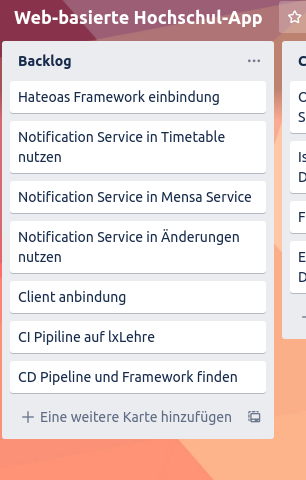
\includegraphics[width=5 cm]{Bilder/Kapitel_2/backlog.png}
\caption{Trello Board Backlog\label{fig:trello_backlog}}
\end{figure}

\subsection*{Planung eines Sprints}

Am Anfang eines jeden Sprints müssen die wichtigsten Aufgaben aus dem Backlog in das Sprint Backlog übernommen werden. Hier ist stets zu beachten, dass dabei möglichst nicht mehr Aufgaben übernommen werden, als im Sprint-Zeitraum erledigt werden können. 

\begin{figure}[H]
\centering
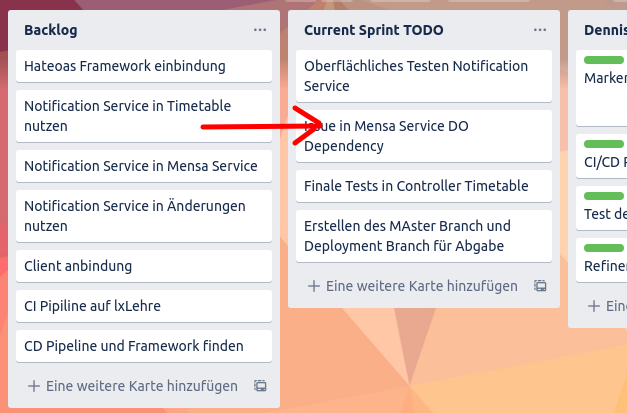
\includegraphics[width=10 cm]{Bilder/Kapitel_2/sprint_backlog.png}
\caption{Trello Board Sprint Backlog\label{fig:trello_sprint_backlog}}
\end{figure}

Innerhalb des Sprint Backlog sollte nun die Aufgaben nach ihrem Zeitaufwand bewertet werden. Die Entwickler entnehmen dem Sprint Backlog die Aufgaben geordnet nach der Priorisierung, die wichtigsten Aufgaben müssen dabei immer zuerst erledigt werden. Die Aufgaben, die am Ende eines Sprints noch nicht aus dem Sprint Backlog entnommen wurden müssen in den nächsten Sprint übernommen werden.

\subsection*{Verteilen der Aufgaben}

Wie bereits erwähnt entnehmen die Entwickler, sobald sie Zeit zur Verfügung haben, eine Aufgabe aus dem Sprint Backlog und hinterlegen sie in ihrer \textit{Todo}-Liste. Von dort aus sollten die Aufgaben mit dem entsprechenden Label versehen werden, das anzeigt, wem die Aufgabe initial zugeordnet wurde. So ist am Ende auch zu erkennen, wer welche Aufgaben erledigt hat.

\begin{figure}[H]
\centering
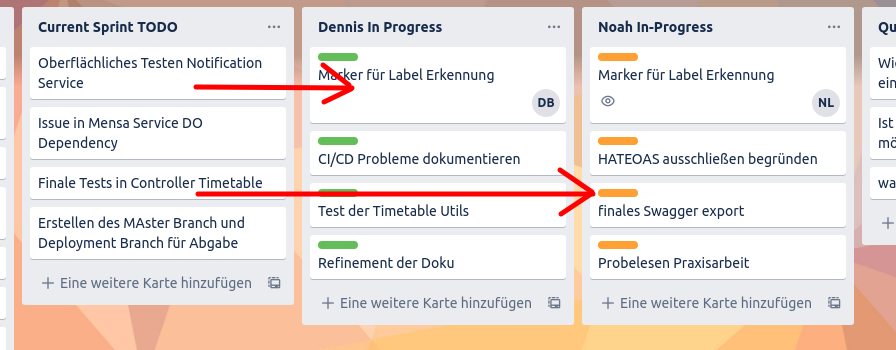
\includegraphics[width=14 cm]{Bilder/Kapitel_2/user_boards.png}
\caption{Trello Board Entwickler Todo Listen\label{fig:trello_user_boards}}
\end{figure}

Anders als im Sprint Backlog ist hierbei darauf zu achten, dass am Ende eines Sprints keine Aufgaben mehr in den Todo-Listen der Entwickler übrig sind. Diese führen sonst auf Dauer nur dazu, dass der Überblick über das Board verloren geht, was das Trello Board im Allgemeinen überflüssig machen würde. Es können allerdings jederzeit mehrere Aufgaben übernommen werden, insofern es sinnvoll ist, diese parallel zu bearbeiten.

\subsection*{Abschluss von Aufgaben}

Sobald eine der Aufgaben erledigt und getestet ist, können die Entwickler sie in die Spalte \textit{Done} übernehmen, in welcher die Aufgaben als endgültig erledigt markiert werden. 

\begin{figure}[H]
\centering
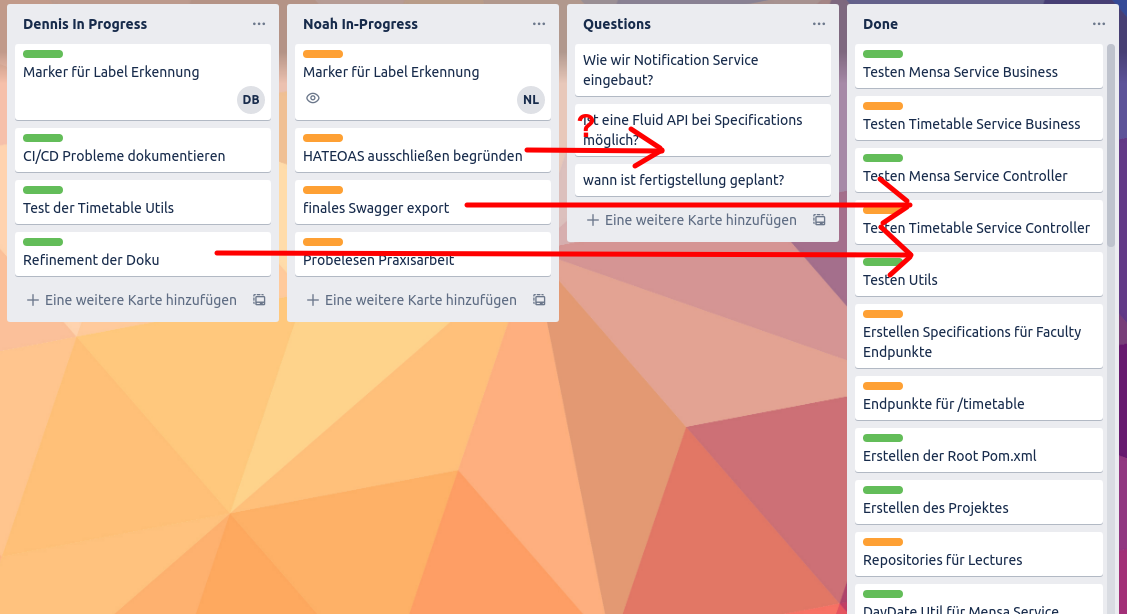
\includegraphics[width=14 cm]{Bilder/Kapitel_2/done.png}
\caption{Trello Board Liste der fertigen Aufgaben\label{fig:trello_done}}
\end{figure}

Sollten während der Bearbeitung jedoch noch Fragen auftreten, welche die Weiterarbeit oder den Abschluss der Aufgabe verhindern, so können die Fragen als einzelne Karte in die Spalte \textit{Questions} erstellt werden. Wenn die Weiterarbeit an einer Aufgabe bis zur Beantwortung der Frage nicht möglich ist, so kann man die Aufgabe auch als Ganzes in die Spalte \textit{Questions} verschieben.\\
\linebreak
Abschließend ist zur Organisation des Projektes zu sagen, dass viele Ansprüche und Konzepte, die \textit{Scrum} mit sich bringt, in einem Team von zwei Entwicklern nicht sinnvoll sind. Dennoch sollte die Grundidee aufgenommen werden, um eine Struktur in der Entwicklung beizubehalten und um wichtige Aufgaben nicht zu vergessen. Dies ist durch die abgewandelte Nutzung des \textit{Scrum}-Konzepts gelungen.